\chapter{Looking for Epistasis in \emph{EvoTSC}}

The results obtained with the \emph{EvoTSC} model that I have presented up until now tackle the regulatory role that DNA supercoiling plays in bacterial genomes.
In this chapter, I return to the idea of epistasis between mutations in the supercoiling level and other mutations that was the root question of the research agenda of my PhD, but within the frame of \emph{EvoTSC}.
In the experiments conducted with \emph{Aevol} and presented in Chapter~\ref{chap:aevol}, one of the reasons for which I was not able to detect a signal of epistasis was that the supercoiling model was too simple, and that supercoiling mutations would not generate interesting paths to explore the fitness landscape.
In \emph{EvoTSC}, supercoiling is on the contrary sufficiently finely modeled to allow the evolution of regulatory networks based on local variations in the level of supercoiling, as I demonstrated in the previous chapters.
Allowing the basal supercoiling level to evolve in some \emph{EvoTSC} populations could therefore arguably, unlike in \emph{Aevol}, generate evolutionary trajectories that allow them to reach higher fitness peaks faster than populations with a constant basal supercoiling level.
In this chapter, I present an experiment that aims at evaluating this hypothesis.

\section{Experimental Setup}

The experiment consists in two successive sets of evolutionary runs.
I first evolved two groups of populations, for 1,000,000 generations, in order to obtain \emph{wild-type} evolved individuals.
The first set does not have supercoiling mutations and consists in the 30 populations described in Chapter~\ref{chap:ploscb}, and the second set comprises 10 fresh populations with supercoiling mutations.
Then, I picked the best individual at the end of the evolution of 5 arbitrarily chosen wild-type populations, and subjected each of these wild-type individuals to a set of environmental shocks, by reassigning new types at random to a proportion of their genes.
For each wild-type individual, I created 5 different shocked individuals from that individual, and each time let a population initialized with clones of the shocked individual evolve for 250,000 generations.
This allowed me to compare the speed of evolution after an environmental shock of 25 populations with, and 25 populations without, mutations in the basal supercoiling level.

\subsection{Mutational Operator for the Supercoiling Level}

The mutational operator that I used for the mutations in the basal supercoiling level $\sigma_{basal}$ of individuals is similar to the one I implemented in \emph{Aevol} and that is presented in Section~\ref{sec:aevol:mut-sc}.
When mutating an individual, we decide whether to mutate its basal supercoiling level with a probability $p$, and draw a small change $\delta\sigma_{basal}$ to be added to the supercoiling level according to a normal law $\mathcal{N}(0, s^2)$.
In this experiment, $p=0.1$ and $s^2=0.0001$.

\begin{figure}
\centering
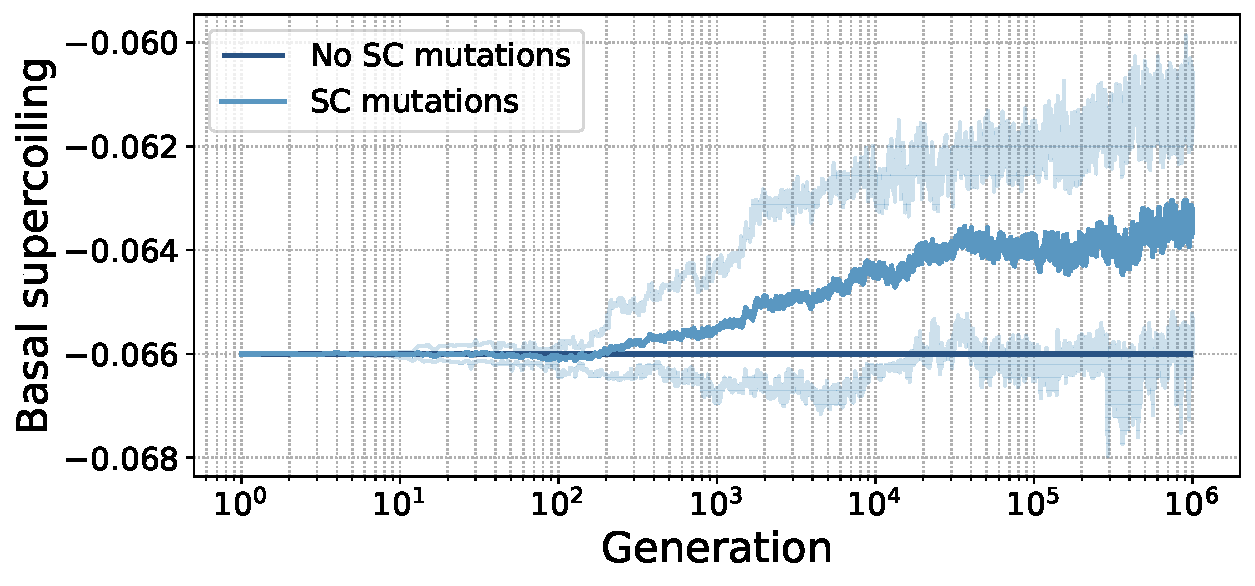
\includegraphics[width=0.75\textwidth]{epistasis/img/basal_sc_all.pdf}
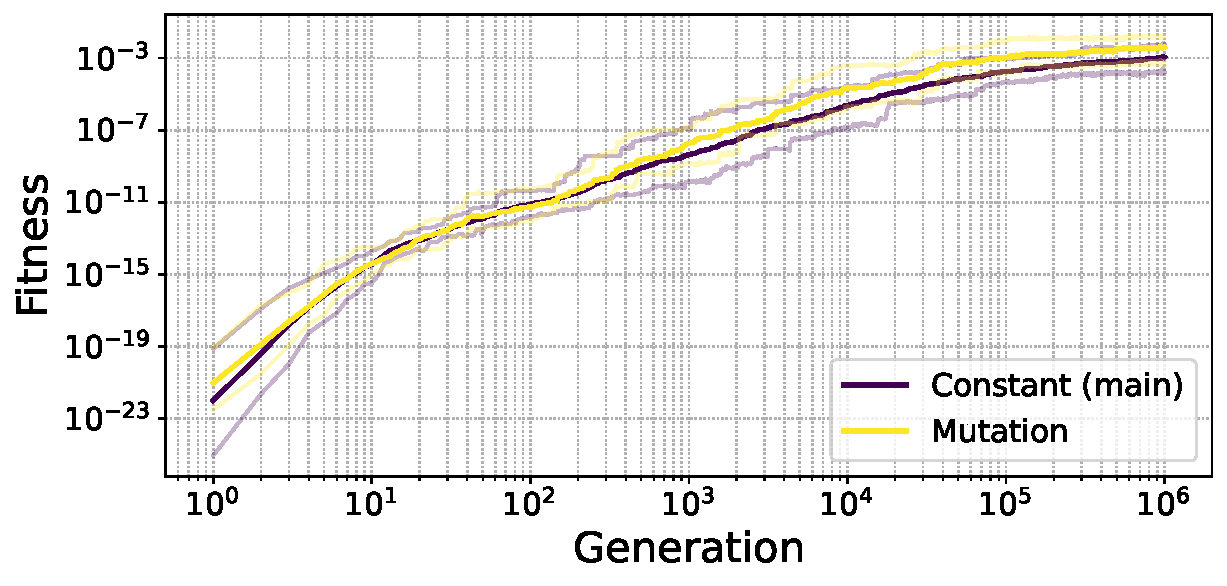
\includegraphics[width=0.75\textwidth]{epistasis/img/fitness_all_with_main.pdf}
\caption[Average basal supercoiling and fitness during evolution of the wild-types, with basal supercoiling level mutations]{Top: average basal supercoiling level of the best individual in every replicate during evolution of the 10 wild-types with (in yellow) and without (in purple) mutations in the basal supercoiling level.
Bottom: average fitness of the best individual in every replicate during evolution, for the wild-types with (yellow) and without (purple) supercoiling mutations.
Lighter lines represent the first and last decile of the data.}
\label{fig:epistasis:wt-evolution}
\end{figure}

Figure~\ref{fig:epistasis:wt-evolution} presents the evolution of the basal supercoiling level (top) and fitness (bottom) of the best individual in each replicate during the evolution of the wild-type populations, with and without supercoiling mutations.
A clear selection pressure towards reducing the amount of negative supercoiling can be observed, as well as a slightly higher fitness throughout evolution of the populations with supercoiling mutations.
A possible hypothesis to explain this higher fitness comes from recalling that, with the initial basal supercoiling level of $\sigma_{basal} = -0.066$, genes tend to have a high expression level, in both environments (see the dash-dotted curve of Figure~\ref{fig:ploscb:activity-by-sigma}).
In that case, decreasing the level of negative supercoiling lessens the bias towards high gene expression in both environments, and therefore helps the inhibition of \emph{A} genes in environment B in these populations (data not shown).

\subsection{Environmental Shock}

\begin{figure}
  \centering
  \begin{elasticrow}[width=\textwidth]
  \elasticfigure{epistasis/img/init_indiv_with-sc00_env_A.pdf}
  \elasticfigure{epistasis/img/init_indiv_rep02_env_A.pdf}
  \end{elasticrow}
  \caption[Evolved wild-type individual before and after an environmental shock]{Genome of one of the control wild-types (left), and shocked individual created from that individual (right), both evaluated in environment A.}
  \label{fig:epistasis:shock}
\end{figure}

In order to simulate an environmental shock on a given individual, we assign a new type at random to 50\% of the genes of that individual (also chosen at random), ensuring that the number of genes of each type remains constant.
This represents the fact that some genes that had to be activated in the old environment must now be inhibited in the new environment, and vice versa.
A representative example of environmental shock is depicted in Figure~\ref{fig:epistasis:shock}.
On the left-hand side is the genome of an evolved wild-type individual, and on the right-hand side is the result of applying an environmental shock to this individual.
The type (color) of one third of the genes changes, but not the local supercoiling level along the genome, as the gene positions themselves remain unchanged.
As a result, a certain number of genes are wrongly activated or inhibited, opening the door to compensatory mutations.

\section{Results}

